% !TEX encoding = UTF-8
% !TEX TS-program = pdflatex
% !TEX root = ../tesi.tex

%**************************************************************
\chapter{Data collection}
\label{cap:data-collection}
In this chapter all the developed analysis tools will be explain.
\\\\For data collection, it wouldn't have been required to develop special tools.
Nevertheless, they have been implemented because they are useful and, above all, usable even in contexts where the amount of data collected is considerably greater.\\\\
Moreover, it was preferred to develop separate tools that perform individual analysis functions. This was done thinking about the fact that these tools could also be used individually in the future in contexts where it will not be necessary to follow a chronological order of execution every time.
\\\\
In addition, a \textit{time control system} has been developed: the analysis tools also keep track of the date on which they are performed to make visible the trend over time because some victim profiles may accept the friend request later because they previously kept it suspended.\\ Each result of each analysis session is enclosed in a folder named with the date on which the analysis session was carried out.

%**************************************************************
\section{Analyze victims: \texttt{victims-analysis.py} tool}
\label{cap:victims-analysis}
To determine the evolution of the \texttt {victims.json} dataset growth during the execution of the \texttt {classificator-profile.py} tool (details in chapter \ref{cap:classificator-profiles}, it was created a simple tool, called \texttt{victims-analysis.py}.\\\\
This tool show on the terminal how many profiles for each category of victim profiles have been saved up to then in the \texttt{victims.json} dataset. \\\\
Furthermore, to make distribution more intuitive, it shows (but not save) a bar graph that highlights the difference in the victim profiles collected for each category. \\\\
This tool was very useful during the execution of the \texttt{classificator-profile.py} tool because it allowed to keep under constant control the trend of the dataset, and, above all, to be able to check that every category will reach the minimum value. 
\begin{center}
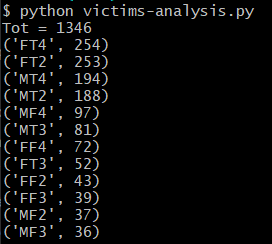
\includegraphics[height=4.5cm]{immagini/cmd-victims-analysis.png}\quad	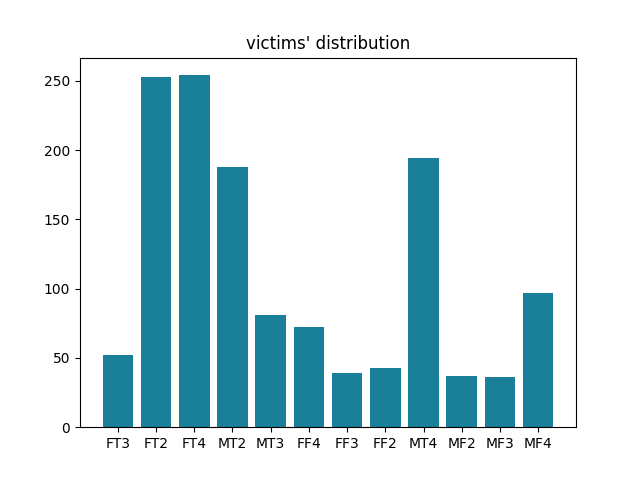
\includegraphics[height=5.25cm]{immagini/victims-analysis-distributiom.png}
\end{center}
Looking at this image it is immediately apparent that the dataset is heavily unbalanced. This situation is discuss in detailed in chapter \ref{cap:discuss-dataset-victims}.

\section{Analyze outcomes of friend requests}
After sending all the friend requests with each attacking profile, we started to launch these various analysis tools.
To do this as automatically as possible, a series of tools have been created, each based on its specific functionality.
\\The developed tools are:
\begin{enumerate}
	\item \texttt{cleaning-save-distribution.py};
	\item \texttt{analyze-friend-requests.py};
	\item \texttt{get-distribution.py};
	\item \texttt{report-acceptance.py}.
\end{enumerate}
These tools must be run in exactly this order each time. Now they will be explain.
\subsection{The tool: \texttt{clean-save-distribution-contents.py}}
This first simple tool cleans the contents of the \texttt{save\_distribution.json}, i.e. it will set its each value to 0.\\
Considering that these tools must be run one after the other on each analysis session, this particular tool must be run first because it modifies the starting file for the analysis.\\
If it contains data from previous analysis sessions, it is invalid because the data would overlap. So, with this tool, the content of this dataset is cleaned up as if it had just been created and therefore ready to accept the new data for a new analysis session.\\\\
Although the function is small, this mini tool was created separately, as it could be used at any time (for example if some error occurs during the analysis).\\\\
Potentially, this tool could also be run only at the end of each analysis session. The important thing is that every time a new analysis session begins, \texttt{save\_distribution.json} dataset must be cleaned.

\subsection{The tool: \texttt{analyze-friend-requests.py}}
This tool verifies for each attacking profile which of the victim profiles has accepted the friend request.\\
Using a list with all the identification codes of the attacking profiles, it fetch the information necessary to log in on Facebook and then it save the list of friends' URLs in a temporary file.\\A function will read the temporary file line by line and find a match with a URL in the \texttt{request-log.json} file in the section dedicated to the attacking profile under consideration. For each profile found, will increase the count inside the \texttt{save\_distribution.json} file, so that at the end of the analysis of each attacking profile, it is possible to see, for each victim, how many and what type of profiles attackers accepted the friend request.\\\\
In the end, It also will show in the terminal how many friend requests have been accepted out of the total of those sent.

\subsection{The tool: \texttt{get-distribution.py}}
\label{cap:distribution-update}
This tool shows the distribution of the friend requests accepted: for each victim, it creates a graph that displays how many friend requests the victim accepted and from which attacker profiles they came from.\\
The tool will first create a folder called "report" with the date the tool is started (for example "report-2021-08-02").\\
Then, inside it will save bar graphs that show this information.\\
Each image contains a graphic about a specific victim and is saved with today's date and victim type (for example "2021-08-02 - 7-MT3").\\
Furthermore, it creates \texttt{distribution\_}\textit{current\_date}\texttt{.json} dataset and update the content of \texttt{distribution\_update.json} dataset, with the report of the data in \texttt{JSON} struct. They are the same file, but the first one is useful to see the report during the time, the last one will be use to have the last updated data to create the \textit{model of acceptance} (details in \ref{cap:model-of-acceptance})\\\\
The graph shown below is an example.\\
It represents how many "MT3" victims, ie males over the age of 50 and with a real profile picture, accepted the friend request and which profiles they came from.\\
\begin{center}
	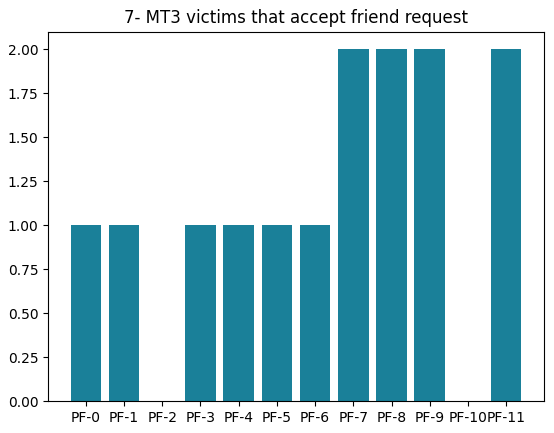
\includegraphics[width=7.5cm]{immagini/2021-08-02 - 7-MT3.png} 
\end{center}
\subsection{The tool: \texttt{report-acceptance.py}}
The last tool to run, called "\texttt{report-acceptance.py}", focuses on the attacker who made the friend request.\\\\
First of all, it creates a folder called \texttt{"report-request"} where it saves a bar chart for each attacking profile showing, for each category of victim profile, how many requests have been made by that attacking profile. \\In this case study, it would not be necessary considering that there are 3 friend requests for each victim profile, but if you have to work with more data this function will be needed again.
\\Then, it will create a second folder, called "\texttt{report-acceptance}", where it saves a bar chart for each attacking profile, showing, for each category of victim profile, how many requests have been accepted to that attacking profile.
\\It will also save this information in the\texttt{distribution\_data} file where \emph{data} means the date the tool was executed (for example "\texttt{distribution\_2021-08-02}").
\\\\An example is a graph below, inserted by the tool in the \texttt{"report-acceptance"} folder, which represents how many victims (and which category they belong to) have accepted the friendship to \texttt{PF-0}, that is the attacking profile with the label \texttt{"MT4"}.\\
\begin{center}
	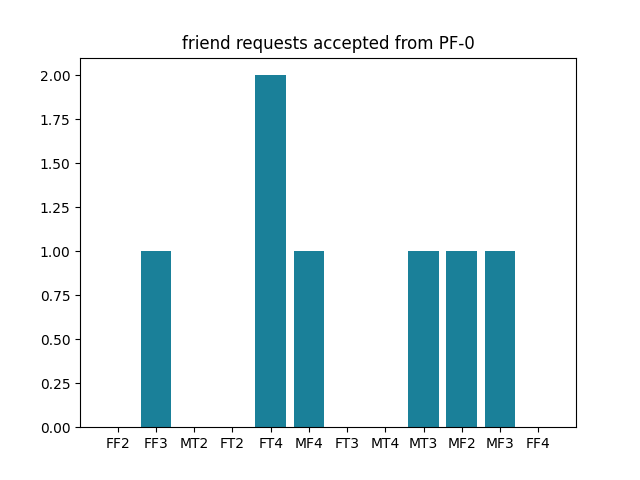
\includegraphics[width=9.5cm]{immagini/PF-0_report-acceptance.png} 
\end{center}